\documentclass[letterpaper,10pt]{article}
\usepackage{graphicx}
\usepackage{listings}
\usepackage{url}

\title{Angular contact with TensorFlow}
\author{DHBW Mosbach/Bad Mergentheim - Rocco Malisi}

\begin{document}
	\maketitle
	\newpage
		
	\begin{abstract}
	Angular contact ball bearings (ACBB) are used in mechanical systems, where their reliability and performance are often critical. Being able to accurately predict the lifetime of ACBBs is important to provide optimal maintenance and avoid failures. This project is about building a model which is able to predict the lifetime of a ACBB. 
	\\ The model is built as a simple neural network using the TensorFlow framework. The data basis is real-world ACBB operational data, containing the rotational speed and radial force as input parameters. 
	\\ To evaluate the models performance, the mean average percentage error (MAPE) metric is used. When comparing the predictions made by the model to actual data, the MAPE metric shows an error of 68 percent.
	\\ Future work involves performing additional data preprocessing and exploring different structures and types of neural networks in order to increase the accuracy of the model.
	
	\end{abstract}
	\newpage
	
	\tableofcontents
	\newpage
	
	\section{Introduction}
	\subsection{Exploratory Data Analysis}
	Exploratory Data Analysis (EDA) is a subdomain of statistics which was first introduced by John W. Tukey in 1977.\cite{tukey} EDA focuses on formulating new hypothesis on basis of the dataset rather than only verifying already existing assumptions. The two major methods when performing EDA are visual and quantitative analysis. Visual analysis is done using plots and diagrams, e.g. boxplots and histograms. Quantitative analysis using procedures like median polish is only done sparingly.
	\subsection{Python tools and libraries for machine learning}
	This section introduces the python tools and libraries used in this project. \\
	\textbf{TensorFlow}: \\ TensorFlow is an open-source machine learning framework developed by Google. It offers simple ways to build, train and deploy models. TensorFlow has powerful and complex functionalities like distributed computing and visualization, but for this project it will only be used to build neural networks.\cite{tensorflow2015-whitepaper} \\
	\textbf{Jupyter}: \\ Jupyter is an open-source library which is mostly used in Data Science. It features notebooks, which are documents combining code, text and visualizations. Code is executed in cells which can be run individually or in specific orders in order to make working with different resources easier.\cite{jupyter} \\
	\textbf{pandas}: pandas is an open-source python library providing high-performance, easy-to-use data structures and data analysis tools. It is mostly used for data preprocessing, data exploration and input/output of data.\cite{pandas} \\
	\textbf{Matplotlib}: Matplotlib is a python library for creating static, animated and interactive visualizations. It features a wide range of plot types and layouts. Matplotlib also enables exporting high-quality visualizations for publications or presentations.\cite{matplotlib} \\
	\newpage
	\section{Methods}
	The objective of this project is to build a model which predicts the lifetime of an angular contact ball bearing (ACBB). This is achieved through an experimental approach, where a model is built using a real-world dataset. After the dataset is analyzed and understood, a neural network predicting the lifetime is built. The performance of the model is improved by experimenting with type and structure of the network. The goal is to create a model, which predicts the lifetime of the ACBB with high accuracy.  
	\section{Results}
	\subsection{Performing an EDA on the dataset}
	To get a better understanding of the dataset, an EDA is performed. The objective is to identify patterns and relationships in the data. The insights gained by this analysis will be used in building and improving the model.
	\newline The dataset cons s of three columns and 1365 rows. The columns are 'Fr' (radial force in N[Newton]), 'n' (rotational speed in rpm[revolutions per minute]) and 'Lifetime' (lifetime in h[hours]). The dataset does not contain any empty or null values and therefore does not require cleaning.
	\newline Figure 1 shows a plot of column Fr. The value of Fr starts at 200 and is increased by 100 every 35 rows throughout the whole dataset. The final and highest value of Fr is 4000. 
	\newline The column Lifetime is shown in figure 3. The highest value at the first row is 88445568 but it drops rapidly throughout the dataset to just 116 in the last row. Every 35 rows the value has a local peak but then quickly drops again. Figure 2 is a plot of rows 1000 and up which shows that this trend continues all the way throughout the dataset even though it can't be seen when plotting all rows. 
	\newline The column n is shown in figure 4. The value of n follows a pattern which repeats every 35 rows for 39 times. From the starting value of 100, n is  increased linearly to its peak value of 3500, after which it drops back to 100 and the next iteration begins. 
	\newline These findings already give insights about potential relationships of the variables. The peaks in the value of lifetime appear when n is at its lowest at 100. When n increases, the peak in lifetime drops sharply. This could be due to the increased load on the bearing system as n increases. As Fr steadily increases throughout the dataset, the peaks of lifetime become smaller even though n follow the same pattern. Therefore Fr must also have a negative correlation with lifetime.
	\newline Figure 5 shows the correlation matrix of the dataset. Both Fr and n show a weak negative correlation with lifetime of -0.21 and -0.12, respectively. 
	
	\subsection{Building the model}
	This chapter is about building the model on basis of the dataset. It will predict the lifetime of the bearing system using Fr and n as input features. The EDA already showed that the dataset does not require cleaning or further preprocessing.
	\newline This model will be a simple neural network. To improve the models accuracy, the number of hidden layers and the number of neurons per hidden layer were tested in different combinations. The best accuracy in predicting the lifetime was achieved with the following configuration: 
	\begin{itemize}
		\item Input layer with 2 neurons for features Fr and n
		\item First hidden layer with 512 neurons and activation function ReLU
		\item Second hidden layer with 512 neurons and activation function ReLU
		\item Output layer with 1 neuron predicting the value of lifetime
	\end{itemize} 
	\ \\The code used to build the model architecture:
	\begin{lstlisting}
		model = tf.keras.Sequential([
		layers.Dense(512, activation='relu', input_shape=[2]), 
		layers.Dense(512, activation='relu'),  
		layers.Dense(1)
		])
	\end{lstlisting}
	The next step is model compilation which includes defining the loss function, optimizer and metrics. The model uses mean absolute percentage error as its loss function, the Adam algorithm as its optimizer and mean average percentage error as evaluation metric. 
	\\ \\ The code used to compile the model:
	\begin{lstlisting}
		model.compile(loss='mean_absolute_percentage_error',
		optimizer=tf.keras.optimizers.Adam(),
		metrics=[tf.keras.metrics.MeanAbsolutePercentageError()],
		run_eagerly=True)
	\end{lstlisting}
	In the final step, the dataset will be prepared and used for training and evaluating the model. First the dataset is split up into training and test data using the scikit-learn train\textunderscore test\textunderscore split function with a train\textunderscore size of 0.8 and a test\textunderscore size of 0.2. The split data is then used to train and evaluate the model. The mean absolute error metric is used to evaluate the model.
	\newpage
	The code to train and evaluate the model:
	\begin{lstlisting}
		X_train, X_test, y_train, y_test = 
		train_test_split(dataset[['Fr', 'n']], dataset['Lifetime'], 
		shuffle=True, 
		train_size=0.8, 
		test_size=0.2)
		
		model.fit(X_train, y_train, epochs=10, verbose=0)
		
		test_loss = model.evaluate(X_test, y_test)
	\end{lstlisting} 
	The evaluation error of this model is 68\% using the mean average percentage error metric. This means that the models predicted value of lifetime is off by 68\% on average.
	
	\begin{figure}
		\caption{Plot of Fr}
		\centering
		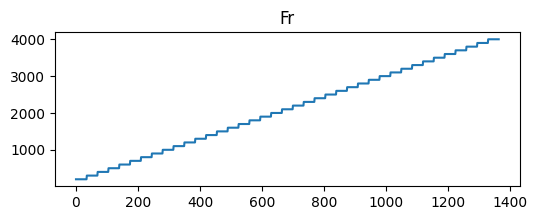
\includegraphics[scale=0.65]{assets/dataset1_column_Fr_plot.png}
	\end{figure}
	\begin{figure}
		\caption{Plot of Lifetime}
		\centering
		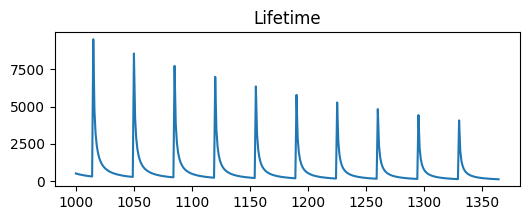
\includegraphics[scale=0.65]{assets/dataset1_column_Lifetime_plot2.png}
	\end{figure}
	\begin{figure}
		\caption{Plot of Lifetime}
		\centering
		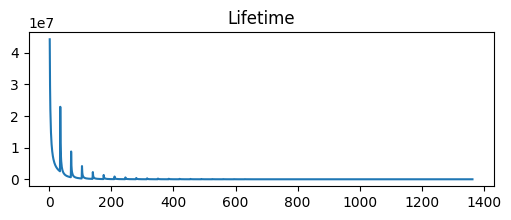
\includegraphics[scale=0.65]{assets/dataset1_column_Lifetime_plot1.png}
	\end{figure}
	\begin{figure}
		\caption{Plot of n}
		\centering
		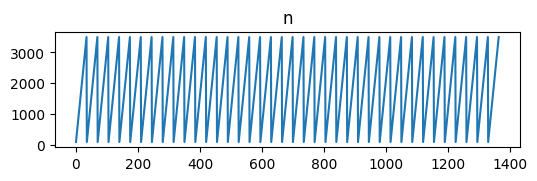
\includegraphics[scale=0.65]{assets/dataset1_column_n_plot.png}
	\end{figure}
	\begin{figure}
		\caption{Correlation matrix of dataset \#1}
		\centering
		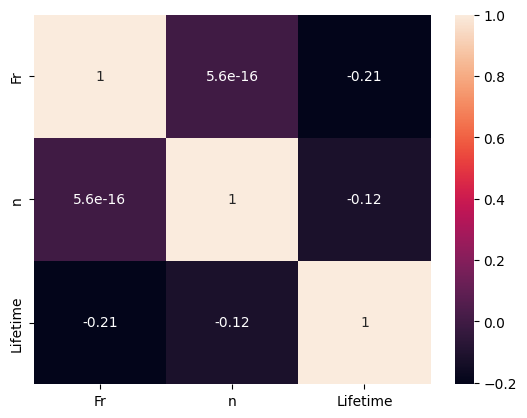
\includegraphics[scale=0.5]{assets/dataset1_correlation_matrix.png}
	\end{figure}
	
	\newpage
	\section{Conclusion}
	The objective of this project was to build a model that is able to accurately predict the lifetime of a ACBB. A simple neural network was built and trained using the real-world dataset. By experimenting with the structure of the network and measuring its performance with the MAPE metric, the best model had an error of 68 percent. This shows that a model predicting the lifetime can be built using the rotational speed and radial force as input features. However, the high error of 68 percent shows, that further data preprocessing or a different neural network structure is necessary in order to improve the performance of the model. In conclusion, this project shows that is it possible to predict the lifetime of a ACBB using a model. In order to use such a model in real-world applications, the performance must first be improved significantly.

	\newpage
	\bibliographystyle{plain} 
	\bibliography{bibliography}
	
\end{document}